\documentclass[simplex.tex]{subfiles}
% NO NEED TO INPUT PREAMBLES HERE
% packages are inherited; you can compile this on its own

\onlyinsubfile{
\title{NeuroData SIMPLEX Report: Subfile}
}

\begin{document}
\onlyinsubfile{
\maketitle
\thispagestyle{empty}

The following report documents the progress made by the labs of Randal~Burns and Joshua~T.~Vogelstein at Johns Hopkins University towards goals set by the DARPA SIMPLEX grant.

%%%% Table of Contents
\tableofcontents

%%%% Publications
\bibliographystyle{IEEEtran}
\begin{spacing}{0.5}
\section*{Publications, Presentations, and Talks}
\vspace{-20pt}
\nocite{*}
{\footnotesize	\bibliography{simplex}}
\end{spacing}
%%%% End Publications
}


\subsection{ndmg}

In an effort to further verify that derivatives produced by the ndmg pipeline are high-quality and execution of a
given dataset within the pipeline was successful, we have expanded upon a automatically generated set of quality
control figures. In particular, we have developed the first, to our knowledge, connectome-specific graph quality
control plot. This figure, shown as the "Degree" panel in Figure~\ref{fig:ndmgqc}, considers the intra- and inter-
hemispheric connectivity of the graph, and plots the degree of each node for both same and across hemispheric
connectivity. Many real-world graphs contain node and edge attributes, but often location is not among them (or it
is used to define the edges); in connectomics, location is an important feature of each node and plays a role in its
connectivity patterns, as in whether a connection will exist within or across hemispheres of the brain. We also are
computing the mean connectome for the given dataset in this summary figure.

\begin{figure}[h!]
\begin{cframed}
\centering
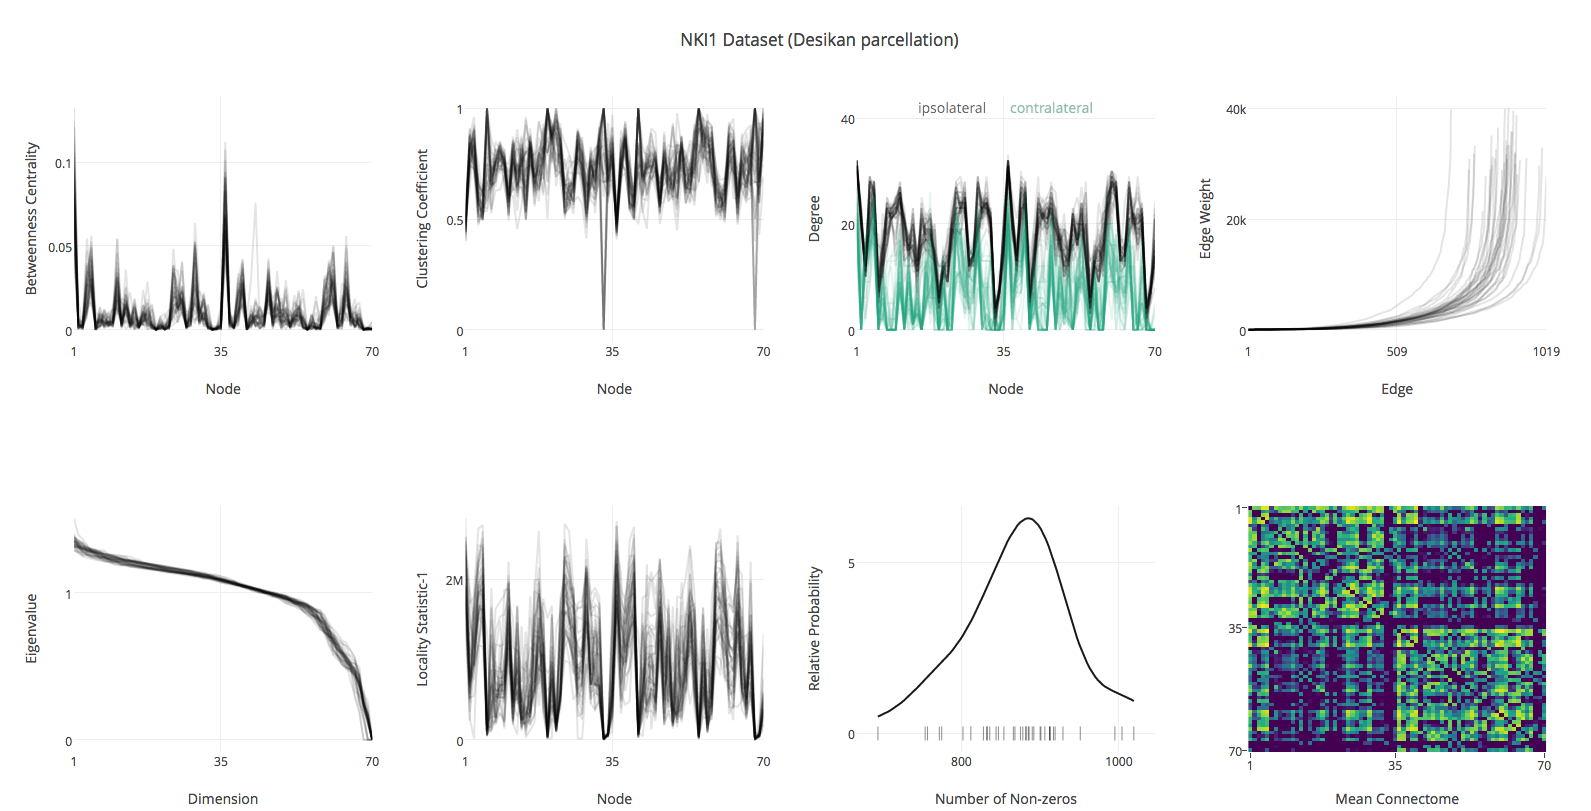
\includegraphics[width=0.95\textwidth]{../../figs/ndmgqcnew.png}
\caption{Quality Control of Connectomes}
\label{fig:ndmgqc}
\end{cframed}
\end{figure}
\end{document}
